\section{Versuchsaufbau und Durchführung}
\label{sec:Versuchaufbau}

Zunächst wird die Probe auf 60°C erhitzt und am externen elektrischen Feld
eine Spannung von $1\,$kV angelegt, welches zur Ausrichtung der Dipole
führt und 15 min gewartet. Danach werden die nun ausgerichteten Dipole
mittels flüssigen Stickstoff eingefroren. Dieses geschieht
bei einer Temeperatur von ca -60°C. Jetzt kann das elektrische Feld
ausgeschaltet werden und die Kondensatorplatten werden kurzgeschaltet um
sich komplett zu entladen. Anschließend kann der Messprozess beginnen,
dafür wird ein Pico-Ampermeter angeschlossen und die Probe mit einer
konstanten Heizrate von $2°C/$min gehitzt und der entstehende Strom notiert.
Anschließend wird diese Messvorgang mit einer Heizrate von $1.5°C/$min
wiederholt.
\begin{figure}
\centering
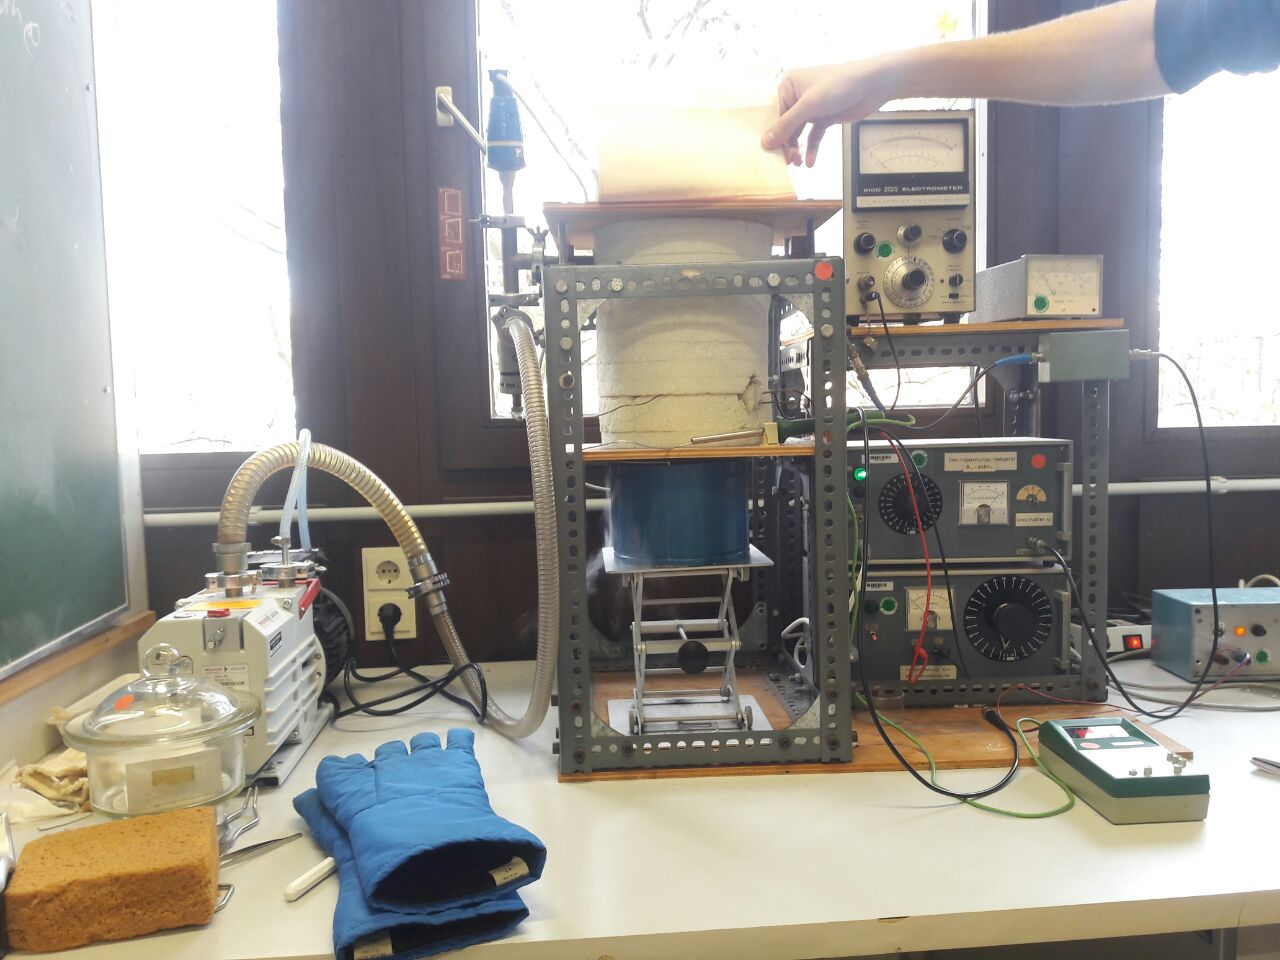
\includegraphics[width=0.8\textwidth]{ressources/photo5458414829602712357.jpg}
\caption{Foto des Versuchsaufbaus}
\label{aufbau}
\end{figure}
